\documentclass[12pt]{article}
\usepackage[czech]{babel}
\usepackage[utf8]{inputenc}
\usepackage[IL2]{fontenc}
\usepackage{wrapfig}
\usepackage{graphicx}
\usepackage{cprotect}
\usepackage[unicode, hidelinks]{hyperref}
\usepackage{amsmath}
\usepackage{tikz}
\usetikzlibrary{arrows,positioning,shapes.geometric, fit, trees, calc}
\usepackage{pgfplots}
\usepgfplotslibrary{external}
\usepackage[capposition=bottom]{floatrow}
\usepackage[bottom]{footmisc}
\usepackage{subcaption}
\usepackage{algorithm2e}
\usepackage{colortbl}

\pgfplotsset{compat=1.15}

\begin{document}
%\catcode`\-=12 % dash for commands (table) BABEL CZ error

%\setlength{\parindent}{0pt}
\begin{titlepage}

\includegraphics[scale=0.2, trim=5cm 0 0 30cm]{logo.jpg}
\begin{center}
\vspace{5cm}
{\Huge
\textbf{KIV/UPS}\\
\vspace{1cm}
}
{\Large
\textbf{Hra oko bere}
}
\end{center}
\vspace{\fill}

\begin{minipage}[t]{5cm}
\flushleft
Martin Hamet\\
A14B0254P\\
hamet@students.zcu.cz
\end{minipage}
\hfill
\begin{minipage}[t]{7cm}
\flushright
\today
\end{minipage}
\end{titlepage}

\tableofcontents
\newpage
\section{Zadání}
\begin{itemize}
\setlength\itemsep{1px}
\renewcommand\labelitemi{--}
\item Implementujte hru "Oko bere". Server bude implementován v jazyce C a klient bude v Java.
\item Komunikace bude realizována nešifrovaným protokolem nad TCP protokolem.
\item Výstupy serveru budou v alfanumerické podobě.
\item Server bude běžet na operačním systému Linux.
\item Server musí být schopen obsluhovat více klientů současně.
\item Musí být možné zachytit proces komunikace na úrovni aplikačního a protokolu a výpis do souboru.
\item Dále budou implementovány statistiky o činnosti serveru.
\end{itemize}

\section{Analýza}
Aby bylo možné zpracovávat více klientů najednou bude vhodné pro každou hru vytvořit vlastní samostatnou herní místnost, která bude obsluhována jedním vláknem. K této místnosti s omezeným počtem hráčů bude umožněno připojování jednotlivých klientů. 

\section{Úvod}
S popularitou digitálních zařízení, která jsou schopna pořizovat fotografie, značně roste sdílení informací ve formě obrázků a to především přostřednictvím internetu. Přestože je, již od roku 1990\cite{Relevance_feedback}, vyhledávání snímků poměrně dobře prozkoumanou disciplínou stále se objevují nová použití s novými technologiemi jako například počítačové vidění, expertní systémy, etc. Obvykle bylo vyhledávání založené na datech spojených se obrázkem jako název a tags. Kvalita těchto přidaných dat se značně liší a nemusí být konzistentní s obsahem obrázků, což vede k využití vyhledávání podle vlastního obsahu obrázku. 

Problém při vyhledávání obrázků podle jejich obsahu vzniká na dvou hlavních místech a to schopnost uživatele exaktně vyjádřit svůj požadavek a schopnost systému rozpoznat globální vlastnosti objektu snímku z jeho reprezentace\cite{Recent_advanceCBIR, DeepLearning_comprehensive}. Jinými slovy systém musí být schopen rozpoznat například vlastnosti auta z jednotlivých pixelů snímku. Jedná se tedy o problém rozpoznání záměru ze strany uživatele a vyšší sémantiky vzhledem ke snímku.

Kolem roku 2000 se výzkum zaměřil na dvě nové metody. Využití popisu pomocí lokáních invariantních vlastností \textit{SIFT} a popisu pomocí \textit{bag of words}.

K posledním trendům patří \textit{deep learning}. Jedná se o soubor algoritmů, které se snaží modelovat vyšší úroveň abstrakce obsahu obrázku pomocí mnohavrstvé hierarchické struktury nelineárních transformací. Tato struktura se snaží napodobovat funkci lidského vnímání. Dobrým příkladem \textit{deep learning} jsou neuronové sítě s mnoha skrytými vrstvami. V našem případě budeme testovat využití takové neuronové sítě pro vyhledávání podobných obrázků vzhledem k jejich obsahu.

\section{Analýza}\label{Analysis}

\subsection{Vyhledávání obrázků na základě obsahu}

\paragraph{SIFT}

\subsection{Neuronová síť}
\label{NN}

\begin{wrapfigure}[13]{r}{6cm}
\vspace{-1cm}
\begin{tikzpicture}
[node distance=0.9cm,>=latex', 
block/.style = 
{draw, shape=circle, align=center, minimum size=15pt}]
\linespread{0.9}
\node [block](1){};
\node [block, below=of 1](2){};
\node [block, below=of 2](3){};

\coordinate (M1) at ($(1)!-0.5!(2)$);
\node [block, right=of M1](11){};
\node [block, below=of 11](12){};
\node [block, below=of 12](13){};
\node [block, below=of 13](14){};

\coordinate (M2) at ($(11)!0.5!(12)$);
\node [block, right=of M2](21){};
\node [block, below=of 21](22){};
\node [block, below=of 22](23){};

\node [block, right=of 21](31){};
\node [block, below=of 31](32){};
\node [block, below=of 32](33){};

\path[draw,->]
(1)edge(11)(1)edge(12)(1)edge(13)(1)edge(14)
(2)edge(11)(2)edge(12)(2)edge(13)(2)edge(14)
(3)edge(11)(3)edge(12)(3)edge(13)(3)edge(14)

(11)edge(21)(11)edge(22)(11)edge(23)
(12)edge(21)(12)edge(22)(12)edge(23)
(13)edge(21)(13)edge(22)(13)edge(23)
(14)edge(21)(14)edge(22)(14)edge(23)

(21)edge(31)(21)edge(32)(21)edge(33)
(22)edge(31)(22)edge(32)(22)edge(33)
(23)edge(31)(23)edge(32)(23)edge(33)
;

\node[rectangle,draw,dashed, fit=(1)(2)(3)](vst){};
%\node at($(1)+(1.0,0.0)$)[block]{asdasd}
\node at ($(vst)+(-0.0,-3.0)$){\text{vstupní}};

\node[rectangle,draw,dashed, fit=(11)(12)(13)(14)(21)(22)(23)](h){};
\node at ($(h)+(0.0,-3.0)$){\text{skrytá}};

\node[rectangle,draw,dashed, fit=(31)(32)(33)](vyst){};
\node at ($(vyst)+(0.0,-3.0)$){\text{výstupní}};

\end{tikzpicture}
\caption{Vrtvy sítě.}
\label{NN_1}
\end{wrapfigure}

Jedná se o prostředek počítačového učení, kde učíme počítač zadanou úlohu na připravených trénovacích datech. Například v případě rozpoznávání obrázků, kdy se systému předkládá velké množství snímků s předem známým obsahem. Systém tyto vstupy zpracovává a snaží se učit datové vzory odpovídající známým výsledkům.

Samotná síť se skládá z mnoha uzlů (neuronů), které jsou mezi sebou hustě propojeny a tvoří tak vlastní neuronovou síť. Většinou jsou neurony organizovány do vrstev. Síť se obvykle skládá z jedné vstupní, výstupní a jedné nebo více skrytých vrstev. Data procházejí tedy sítí pouze jedním směrem od vstupní k výstupní vrstvě (viz obr.\ref{NN_1}).

Všechny vstupy neuronu mají přidělené váhy a jejich produkt jejich hodnot vstupem aktivační funkce neuronu (například sigmoida). Výstupem jednoho neuronu je tedy hodnota aktivační funkce. Tuto hodnotu $O$ tedy spočítáme jako:
\begin{equation}
\label{eq_activation}
O=S\left( \sum _{ v }^{  }{ {  }_{ i }\cdot { w }_{ i } }  \right)
\end{equation}
kde $v_i$ je hodnotou vstupu $i$ neuronu, $w_i$ je váha příslušná vstupu $i$ a $S$ je aktivační funkce.
 
Na počátku jsou váhy všech vstupů jednotlivých neuronů nastaveny na náhodné hodnoty. V procesu trénování, kdy jsou
do sítě zavedena vstupní data (na neurony ve vstupní vrstvě), transformací vstupních hodnot zatím náhodnými vahami získáme hodnoty aktivačních funkcí ve výstupní vrstvě. Dále je třeba provést samotný akt učení, kdy pomocí zpětné propagace (viz \ref{back_propagation}) upravujeme váhy neuronů tak, aby se výstup více blížil našemu požadovanému. Po dostatečném počtu opakování tohoto procesu bude síť schopná vrátit požadovaný výstup na podobný vstup. 

Vzhledem k tomu že hledáme podobné snímky a nikoliv pouze klasifikaci do nějakých tříd je možné využít hodnoty jednotlivých neuronů v \textit{FCL} jako popisový vektor, který budeme srovnávat s ostatními popisy v databázi, pro získání podobných obrázků.

\subsubsection{Zpětná propagace}
\label{back_propagation}

\subsection{Konvoluční neuronová síť}
Myšlenka konvoluční neuronové sítě \textit{CNN}\footnote{
Convolutional Neural Network} spočívá ve využití předzpracování snímku, které poskytne unikátní pohled na scénu (například při detekci hran). Informace získané tímto způsobem použijeme jako vstup klasické neuronové sítě.

Název \textit{CNN} je odvozen od konvolučního operátoru, který použijeme jako prostředek výše zmíněného předzpracování viz \ref{conv_op}. Obecná CNN je založená na získávání informací z obrázku pomocí těchto konvolučních operátorů (fltrů), které si však sama vytvoří. Kombinací jednotlivých filtrů je síť schopná detekovat netriviální vlastnosti snímku. Jako příklad lze uvést kombinaci filtrů pro detekci horizontálních a vertikálních hran, která by umožnila síti rozpoznávat "rohy" například u dveří. Samozřejmě většinou filtrům, vytvořených vlastní sítí, a jejich kombinacím nelze snadno přiřadit význam srozumitelný člověkem, avšak princip přiřazování významu jednotlivým částem snímku zůstává stejný.

\begin{figure}[h]
\centerline{
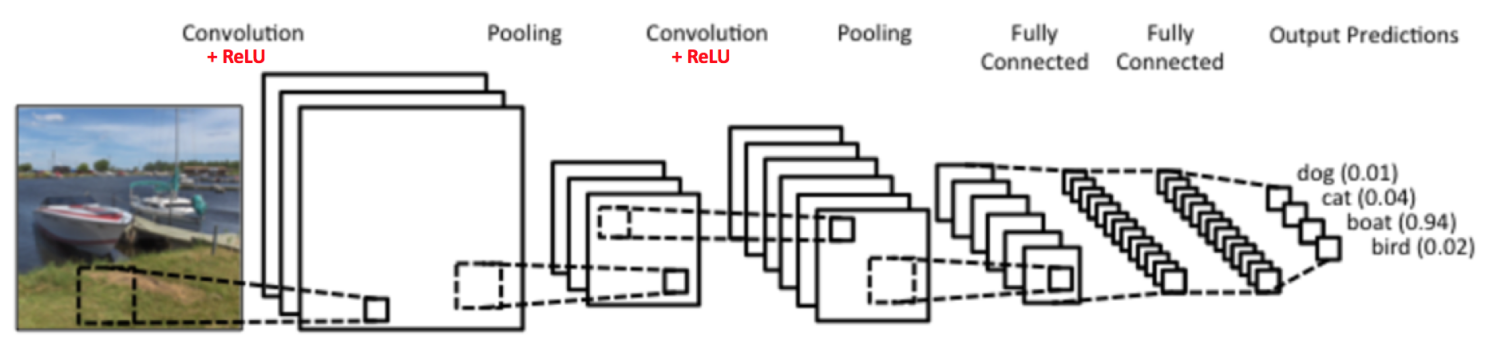
\includegraphics[width=15cm]{CNN_struct.png}
}
\caption[]{Struktura CNN\footnotemark}
\label{im_CNN_structure}
\end{figure}
\footnotetext{
Převzatý obrázek CNN \url{
https://ujwlkarn.files.wordpress.com/2016/08/screen-shot-2016-08-07-at-4-59-29-pm.png?w=1493}
}

Celková struktura CNN je znázorněna na obr.\ref{im_CNN_structure}, kde tato síť obsahuje dvě konvoluční vrstvy za kterými vždy následuje \textit{ReLU}\footnote{Rectified Linear Unit
} a \textit{pooling} a tři plně propojené vrstvy \textit{FCL}\footnote{
Fully Connected Layer
}. Tyto poslední vrstvy představují klasickou neuronovou síť, kde je každý neuron propojen s každým neuronem v následující i předchozí vrstvě jak bylo popsáno výše (\ref{NN} a na obr. \ref{NN_1}). 

\subsubsection{Konvoluční operátor}
\label{conv_op}
Konvoluce je matematická operace nad maticí pomocí jiné matice (jádra). První maticí je v našem případě samotný snímek respektive jeho pixely uspořádané do matice a jádrem bude samotný operátor. Výslednou hodnotu matice získáme ze vztahu:
\begin{equation}
{ F }_{ x,y }=\sum _{ i=-k }^{ k }{ \sum _{ j=-k }^{ k }{ { M }_{ x-i, y-j }\cdot { K }_{ i,j } }  } 
\end{equation}



kde ${ F }_{ x,y }$ je hodnota výsledné matice na pozici $[x,y]$, $k$ je dimenze jádra (jádro musí být čtvercová matice), $M$ je zdrojová matice a $K$ je matice jádra.

Samotný výpočet operace je lépe vidět na příkladu (viz obr.\ref{conv_cnv}).

\begin{figure}[h]
\tikzset{highlight/.style=
{rectangle,fill=black!25, rounded corners ,draw,fill opacity=0.5,thick,inner sep=0pt}}

%mark
\newcommand{\tikzmark}[2][name]{%
\tikz[overlay,remember picture, baseline=(#1.base)] \node (#1) {#2};
}
%highlight submatrix
\newcommand{\Highlight}[2][nodename]{%
\tikz[overlay,remember picture]{%
\node[highlight,#2] (#1) {};}}

\[
K=\left[
\begin{array}{*4c}
0&1&0\\
1&-4&1\\
0&1&0
\end{array}\right]
M=\left[
\begin{array}{*5{c}}
\tikzmark[ltop]{1} & 2 & 1 & 2 & 5\\
1 & 3 & 3 & 4 & 8\\
2 & 2 & \tikzmark[rbot]{\tikzmark[ltop2]{3}} & 5 & 5\\
1 & 2 & 5 & 4 & 5\\
4 & 5 & 3 & 5 & \tikzmark[rbot2]{4}
\end{array}
\right]
\]

\vspace{-0.5cm}

\[
\tikzmark[single3]{$F_{22}$}\hspace{0.3cm}=
\left(\begin{array}{*4c}
0+ & 1\cdot 2+ & 0+\\
1\cdot 1+& -4\cdot 3+ & 1\cdot 3+\\
0+ & 1\cdot 2+ & 0
\end{array}\right)
=-4
\hspace{0.5cm}%
F=\left[
\begin{array}{*5c}
 &  &  &  & \\
 & \tikzmark[single]{-4} & 0 & 2 & \\
 & 2 & 2 & -4 & \\
 & 5 & -8 & \tikzmark[single2]{0} & \\
 &  &  &  & 
\end{array}\right]
\Highlight[mk1]{fit=(ltop)(rbot)}
\Highlight[f1]{fit=(single)}
\Highlight[mk2]{fit=(ltop2)(rbot2), fill=red}
\Highlight[f2]{fit=(single2), fill=red}
\Highlight[exf1]{fit=(single3)}
\]
\tikz[overlay, remember picture]{
\draw[->,thick,black!50,dashed] (mk1) -- (f1) node [pos=0.66,above] {};
\draw[->,thick,black!50,dashed] (mk1) -- (single3) node [pos=0.66,above] {};
\draw[->,thick,red!50,dashed] (mk2) -- (f2) node [pos=0.66,above] {};
}
\caption{Příklad výpočtu konvoluce}
\label{conv_cnv}
\end{figure}

\begin{wrapfigure}[8]{l}{6cm}
\[
\left[\begin{array}{*4c}
1&1&1\\
0&0&0\\
-1&-1&-1
\end{array}\right]
\]
\caption{Konvoluční filtr pro detekci horizontálních hran}
\label{edge_h}
\end{wrapfigure}
Vhodnou volbou hodnot jádra lze vytvořit filtr například pro detekci horizontálních hran (viz obr.\ref{edge_h}). Při použití takového filtru je třeba ošetřit kraje zdrojové matice buď bude výsledek menší v závislosti na velikosti filtru, nebo lze doplnit původní matici o nulové okraje potřebné pro filtr.

\subsubsection{Nelinearita a \textit{pooling}}

\begin{wrapfigure}[10]{r}{7cm}
\vspace{-0.3cm}
\tikzset{highlight/.style=
{rectangle,fill=black!25, rounded corners ,draw,fill opacity=0.5,thick,inner sep=0pt}}

%mark
\newcommand{\tikzmark}[2][name]{%
\tikz[overlay,remember picture, baseline=(#1.base)] \node (#1) {#2};
}
%highlight submatrix
\newcommand{\Highlight}[2][nodename]{%
\tikz[overlay,remember picture]{%
\node[highlight,#2] (#1) {};}}

\[
\left[
\begin{array}{*4c}
-4 & 0 & 2\\
2 & 2 & -4\\
5 & -8 & 0
\end{array}\right]
\xrightarrow{ReLU}
\left[
\begin{array}{*4c}
0 & 0 & 2\\
\tikzmark[ltop2]{2} & \tikzmark[ltop]{2} & 0\\
5 & \tikzmark[rbot2]{0} & \tikzmark[rbot]{0}\\
\end{array}\right]
\]
\vspace{-0.2cm}
\[
\hspace{2cm}\xrightarrow[2\times 2]{Pooling}
\left[
\begin{array}{*2c}
2 & 2\\
\tikzmark[single2]{5} & \tikzmark[single]{2}
\end{array}\right]
\Highlight[r11]{fit=(ltop)(rbot), fill=red}
\Highlight[r12]{fit=(ltop2)(rbot2)}
\Highlight[p11]{fit=(single), fill=red}
\Highlight[p12]{fit=(single2)}
\]

\tikz[overlay, remember picture]{
\draw[->,thick,red!50,dashed] (r11) -- (p11) node [pos=0.66,above] {};
\draw[->,thick,black!50,dashed] (r12) -- (p12) node [pos=0.66,above] {};
}
\caption{Příklad \textit{ReLU} a následný \textit{pooling}}
\label{conv_rel_pool}
\end{wrapfigure}

Jednotlivé operace konvoluce jsou pouze lineární operace a proto s využitím \textit{ReLU} zavedeme do procesu zpracování nelinearitu, kdy nahradíme všechny záporné hodnoty ve výsledku hodnotou nulovou (viz obr.\ref{conv_rel_pool}). Toto nahrazení také zrychluje učení v případě nulové váhy daného neuronu tento neuron přestává mít jakýkoliv vliv na výstup (není potřeba počítat úpravu jeho váhy).

Proces \textit{pooling} za každou konvolucí se stará o snížení dimenze jednotlivých výstupů z filtrů se zachováním jejich nejdůležitějších součástí. Jedná se tedy o zmenšení výsledné matice, kde definujeme okolí pro každý prvek a z daného okolí bereme pouze maximální hodnotu (viz obr.\ref{conv_rel_pool}).

\subsection{Autoencoder}

\begin{wrapfigure}[13]{r}{8cm}
\vspace{-1cm}
\begin{tikzpicture}
[node distance=0.7cm,>=latex', 
block/.style = 
{draw, shape=circle, align=center, minimum size=15pt}]
\linespread{0.9}
\node [block](1){};
\node [block, below=of 1](2){};
\node [block, below=of 2](3){};
\node [block, below=of 3](4){};

\node [block, right=of 1](11){};
\node [block, below=of 11](12){};
\node [block, below=of 12](13){};
\node [block, below=of 13](14){};

\coordinate (M2) at ($(11)!0.5!(12)$);
\node [block, right=of M2](21){};
\node [block, below=of 21](22){};
\node [block, below=of 22](23){};

\coordinate (M3) at ($(21)!0.5!(22)$);
\node [block, right=of M3](31){};
\node [block, below=of 31](32){};

\coordinate (M4) at ($(31)!-0.5!(32)$);
\node [block, right=of M4](41){};
\node [block, below=of 41](42){};
\node [block, below=of 42](43){};

\coordinate (M5) at ($(41)!-0.5!(42)$);
\node [block, right=of M5](51){};
\node [block, below=of 51](52){};
\node [block, below=of 52](53){};
\node [block, below=of 53](54){};

\node [block, right=of 51](61){};
\node [block, below=of 61](62){};
\node [block, below=of 62](63){};
\node [block, below=of 63](64){};

\path[draw,->, black!50]
(1)edge(11)(1)edge(12)(1)edge(13)(1)edge(14)
(2)edge(11)(2)edge(12)(2)edge(13)(2)edge(14)
(3)edge(11)(3)edge(12)(3)edge(13)(3)edge(14)
(4)edge(11)(4)edge(12)(4)edge(13)(4)edge(14)

(11)edge(21)(11)edge(22)(11)edge(23)
(12)edge(21)(12)edge(22)(12)edge(23)
(13)edge(21)(13)edge(22)(13)edge(23)
(14)edge(21)(14)edge(22)(14)edge(23)

(21)edge(31)(21)edge(32)
(22)edge(31)(22)edge(32)
(23)edge(31)(23)edge(32)

(31)edge(41)(31)edge(42)(31)edge(43)
(32)edge(41)(32)edge(42)(32)edge(43)

(41)edge(51)(41)edge(52)(41)edge(53)(41)edge(54)
(42)edge(51)(42)edge(52)(42)edge(53)(42)edge(54)
(43)edge(51)(43)edge(52)(43)edge(53)(43)edge(54)

(51)edge(61)(51)edge(62)(51)edge(63)(51)edge(64)
(52)edge(61)(52)edge(62)(52)edge(63)(52)edge(64)
(53)edge(61)(53)edge(62)(53)edge(63)(53)edge(64)
(54)edge(61)(54)edge(62)(54)edge(63)(54)edge(64)
;

\node[rectangle,draw,dashed, fit=(1)(2)(3)(4)](vst){};
\node at ($(vst)+(-0.0,-2.7)$)(vstA){\text{vstup}};

\node[rectangle,draw,dashed, fit=(61)(62)(63)(64)](vyst){};
\node at ($(vyst)+(-0.0,-2.7)$)(vystA){\text{výstup}};

\node[rectangle,draw, fit=(31)(32)](enc){};
\node at ($(enc)+(0.0,-1.5)$){\text{kód}};

\node[rectangle,draw,dashed, fit=(vst)(vstA)(31)](encoding){};
\node at ($(encoding)+(0.0,3.0)$){\text{kódování}};

\node[rectangle,draw,dashed, fit=(vyst)(vystA)(41)](decoding){};
\node at ($(decoding)+(0.0,3.0)$){\text{dekódování}};

\end{tikzpicture}
\caption{Struktura autoenkoderu}
\label{AE_struct}
\end{wrapfigure}

Jedná se o neuronovou síť určenou pro učení bez učitele. Není tedy nutné předem znát správný výsledek při trénování. Princip funkce autoenkoderu spočívá v učení sítě co nejlépe replikovat vstupní hodnoty na svém výstupu. Tedy poždovaný výstup je vstupní vektor sítě a proto vstupní i výstupní vrstva musí mít stejný počet neuronů. Struktura autoenkoderu se obecně skládá z kódovací a dekódovací části jak je vidět na obr. \ref{AE_struct}. Zpracováním vstupu v kódovací části získáme kódové slovo, které se dekódovací část snaží převést zpět na původní vstup. Výstupem je vzniklý kód a nikoliv  výstupní vrstva, která slouží pouze jako nástroj pro učení. Vytvářením "úzkého hrdla" (vrstvy s menším počtem neuronů) zajistíme ztrátovou kompresi vstupu a nutíme tím síť k vytvoření robustního kódování (odtud název autoenkoder) ze kterého bude možné co nejlépe sestavit původní vstup.

V kombinaci s konvolucí resp. CNN se autoenkoder snaží najít kódování snímku pomocí jednotlivých filtrů, tedy popis snímku pomocí jeho význačných vlastností. Takto vzniklý kód by měl obsahovat zobecněný popis snímku, který bude možné použít pro porovnání a výběr podobných snímků.

\subsection{Datové sady obrázků}


%Ukázka



\paragraph{Caltech 101(256)\cite{caltech101}\cite{caltech256_report}}
Jedná se o databázi čítající $9\,000$($30\,000$) obrázků dělených do 101(256) kategorií. Obrázky byly pořízeny s využitím \textit{Google Image Search} a ručně roztříděny do kategorií. Kategorie průměrně obsahují 90 (119) prvků. Jednotlivé snímky jsou průměrně rozměrů $300\times 200$pixelů.

\paragraph{Corel\cite{corel}}
Dataset obsahuje $10\,000$ obrázků rozdělených do $80$ kategorií. Obrázky mají formát $192\times 128$ nebo $128\times 192$, který pevně daným počtem pixelů usnadňuje zpracování.

\paragraph{ImageNet}
Velmi rozsáhlá databáze s více než $15$ miliony obrázků s vysokým rozlišením dělených do $22\,000$ kategorií. Snímky byly získány z webu a ručně řazeny do tříd. Pro zpracování je možné využít podmnožin určených pro pro \textit{ImageNet Large-Scale Visual Recognition Challenge}(ILSVRC)\cite{ILSVRC15}. Nevýhodou jsou různé formáty rozlišení.

\paragraph{CIFAR10}
Soubor se skládá z $60\,000$ obrázků rozdělených do $10$ tříd. Každý snímek je ve formátu $32\times 32$ pixelů. Set obrázků je rozdělen do trénovacích a testovacích podmnožin pro každou třídu. Bylo by možné použít rozšířenou verzi \textit{CIFAR100}.

\subsection{Metrika}
Systémy v oblasti klasifikace a rozpoznávání je třeba nějakým způsobem hodnotit, aby bylo možné vyjádřit jejich úspěšnost. Takové hodnocení umožňuje systém porovnat s konkurencí, nebo zjistit efekt jeho modifikací při vývoji. 

Hlavní otázkou je jakým způsobem systém hodnotit. Z principu rozpoznávání vyplývají dva hlavní měřitelné atributy, úplnost a přesnost (viz \ref{met_recall} resp. \ref{met_precision}).

Protože systémy popsané dvěma atributy není tak snadné porovnávat, v praxi je vhodnější využít popisu pouze jednou hodnotou. Takovou hodnotu je třeba přizpůsobit konkrétní úloze. Pro popis se nabízí několik možností jako užití \textit{F-measure}, průměrná přesnost, střední geometrická přesnost (GMAP), střední průměrná přesnost (MAP), etc.

V našem případě bude výsledkem dotazu seznam obrázků seřazený podle relevance určené systémem. Bude tedy vhodné využít průměrné přesnosti (viz \ref{met_AP}), která zohledňuje pořadí nalezených výsledků. Jak je vidět na obr.\ref{met_example} průměrná přesnost značně zvýhodňuje prvky podle jejich pořadí v odpovědi na dotaz. Pro popis použijeme tedy metriku střední průměrné přesnosti, která zhodnotí výsledky všech použitých dotazů při testování s velkým důrazem na uspořádání získaného výsledku. Bylo by možné použít modifikaci GMAP, která vyžaduje dostatečný výkon ve všech dotazech. Náš systém nebude mít omezení na nejhorší povolenou úspěšnost a nebudeme tedy tuto metriku uvažovat.


\subsubsection{Přesnost}
\label{met_precision}
Přesnost neboli \textit{precision} hodnotí kolik relevantních výsledků systém poskytl. Jedná se o podíl relevantních a všech získaných výsledků (viz rovnice č. \ref{eq_precision}). Procentuální přesnost intuitivně ukazuje úspěšnost rozpoznávání pro daný dotaz. V případě že systém vrátil všechny relevantní výsledky hodnota přesnosti bude $100\%$. Výpočet přesnosti $P@n$ provedeme dle vzorce:

\begin{equation}
\label{eq_precision}
P@n=\frac{ { R }_{ Q } }{ Q }
\end{equation}

kde $Q$ je počet získaných výsledků na dotaz a $R_Q$ je počet relevantních výsledků ze všech získaných. Samotnou přesnost značíme jako $P@n$, kde $n$ udává počet požadovaných výsledků dotazu. Pokud by v datech existoval pouze jeden relevantní výsledek přesnost pro velké $n$ by se značně snížila a bude tedy třeba tento fakt zohlednit.

\subsubsection{Úplnost}
\label{met_recall}
Samotná přesnost nevypovídá o úplnosti dotazu. Jinými slovy chtěli by jsme zohlednit počet všech relevantních prvků ve zdroji. Pro tyto potřeby se používá hodnota úplnosti neboli \textit{recall}. jedná se o poměr získaných relevantních výsledků a všech relevantních prvků v prohledávaném zdroji. Výpočet úplnosti $R@n$ pro dotaz na $n$ prvků provedeme dle vzorce:

\begin{equation}
\label{eq_recall}
R@n=\frac{ { R }_{ Q } }{ R }
\end{equation}

kde $R_Q$ je počet relevantních výsledků ze všech získaných, podobně jako v případě výpočtu \textit{Precision}(viz \ref{met_precision}), a $R$ je počet všech relevantních prvků v databázi.

Hlavní nevýhodou tohoto atributu je nutnost znalosti všech relevantních prvků v databázi na daný dotaz.

\subsubsection{F-míra}
Hodnota \textit{F-measure}\cite{Metrics_fmeasure} udává harmonický průměr úplnosti a přesnosti (viz rovnice č.\ref{eq_fmeasure}). Vztah pro výpočet by bylo možné dále upravit, pokud by jsme chtěli klást větší důraz na přesnost nebo úplnost. Přestože \textit{f-measure} zahrnuje oba výše zmíněné atributy, její hodnotu nelze intuitivně interpretovat a sloužila by pouze jako prostředek pro porovnání s případnou předpojatostí vůči jednomu z atributů.

\begin{equation}
\label{eq_fmeasure}
{ F }_{ 1 }=2\cdot \frac { P\cdot { R }_{ Q } }{ P+{ R }_{ Q } }
\end{equation}

\subsubsection{Průměrná přesnost}
\label{met_AP}
Tato hodnota kombinuje úplnost a přesnost pro daný počet dotazovaných prvků. Průměrná přesnost\cite{Average_precision} $AP@n$ je průměrem hodnot přesností $P@n$ ze všech relevantních výsledků $n$. Hodnotu vypočítáme ze vztahu:

\begin{equation}
AP@n=\cfrac { \sum _{ n }^{  }{ P@n }  }{ R_Q } 
\end{equation}

kde $P@n$ je přesnost pro n požadovaných prvků (viz vzorec č. \ref{eq_precision}) a $R_Q$ je počet získaných relevantních prvků. Příklad výpočtu je vidět na obr. \ref{met_example}.

\paragraph{Střední průměrná přesnost}
\label{met_MAP}
Hodnotou $mAP$ rozumíme pouze průměr jednotlivých průměrných přesností $AP$. Výpočet je znázorněn na obr. \ref{met_example}.

\begin{figure}[h]
Předpokládáme že máme celkem $4$ relevantní prvky pro oba dotazy.

\begin{tabular}{*7c}
Query \#1&F&T&T&F&T&F\\
\begin{small}
$R@n$
\end{small}&
0&0.25&0.50&0.50&0.75&0.75\\
\begin{small}
$P@n$
\end{small}&
0&0.50&0.67&0.50&0.60&0.50\\\\

Query \#2&T&F&T&F&F\\
\begin{small}
$R@n$
\end{small}&
0.25&0.25&0.50&0.50&0.50\\
\begin{small}
$P@n$
\end{small}&
1.00&0.50&0.67&0.50&0.40

\end{tabular}

\floatfoot{
T značí relevantní prvek\\
F značí irelevantní prvek\\
}

\caption{Příklad dotazu}

střední průměrnou hodnotu $mAP$ spočítáme jako:
\begin{equation}
\nonumber
\begin{split}
AP_{Q1} &= {(0.50+0.67+0.60)}/{3}=0.59\\
AP_{Q2} &= {(1.00+0.67)}/{2}=0.83\\
mAP &= {(0.59+0.54)}/{2}=0.71
\end{split}
\end{equation}

\label{met_example}
\end{figure}

\section{Závěr}
Nejpoužívanější metody pro klasifikaci obrázků využívají vlastností snímku. Jedná se o vnější znaky jako "tags", "bag of words", etc. a vnitřní související s vlastním obsahem. V našem případě se zabýváme pouze vnitřními. Problémem zůstává volba metody extrakce takových vlastností, která významně ovlivňuje úspěšnost klasifikace při konkrétní aplikaci systému. Protože hledáme podobné obrázky k danému vzoru v databázi, pouhé určení třídy daného snímku jako v běžném klasifikačním systému je krajně nedostačující popis. Hledáme tedy věrný popis scény, který je ovšem dostatečně obecný pro vyhledání podobných snímků.

Princip konvoluce se ukazuje jako vhodná cesta zkoumání obsahu. V kombinaci s neuronovou sítí dokážeme do jisté míry napodobovat lidské vidění ve smyslu identifikace objektů v závislosti na jejich významných rysech. Konvoluční filtry bude vytvářet samotná \texttt{CNN} ve fázi trénování, odpadá tím náročný úkol výběru vhodné sady a jejich kombinace.

Jako způsob trénování se jeví vhodné sestavit síť jako autoenkodér. Vstup (snímek) bude při trénování i požadovaným výstupem. Jinými slovy síť se bude učit vybírat vlastnosti nastavováním konvolučních filtrů tak, aby byla schopná co nejlépe replikovat stejný snímek na výstupu. Jako popis se tedy nevyužije samotný výstup \texttt{CNN}, ale její část ve, které jsou zakódované vlastnosti snímku. Vzhledem k tomu že se síť učí replikovat snímek na vstupu mělo by se jednat o jeho dobrou reprezentaci.

Výběr datových sad pro zpracování závisel především na rozměrech obrázku, které bude třeba upravit tak, aby odpovídal počet pixelů a počet neuronů vstupní vrstvy. Příliš zásadní úpravy by značně zhoršovali funkčnost rozpoznávání (příliš velké zploštění, roztažení etc.).

Jako metrika určování úspěšnosti systému byla zvolena střední průměrná přesnost, která velice dobře popisuje daný problém a to především vzhledem k pořadí získaných výsledků. Chceme vytvořit systém, který vrátí seznam snímků řazený podle jejich podobnosti vzoru.

%záver - shrnutí ,další postup
%účet- metacentrum

\pagebreak
\bibliography{mybib}
\bibliographystyle{plain}
%\bibliography{References}
\end{document}